\documentclass[12pt]{article}
\usepackage[spanish, es-tabla]{babel}
\usepackage[top=1.78cm, bottom=1.78cm,left=1.65cm, right=1.65cm]{geometry}
\usepackage[utf8x]{inputenc}
\usepackage{amsmath}
\usepackage{graphicx}
\setlength{\parindent}{12pt}
\usepackage[colorinlistoftodos]{todonotes}
\usepackage{multicol}
\let\olditemize\itemize
\def\itemize{\olditemize\itemsep=0pt }
\usepackage[hidelinks]{hyperref}

\usepackage[pages=some]{background}
\backgroundsetup{
 scale=1,
 color=black,
 opacity=0.3,
 angle=0,
 contents={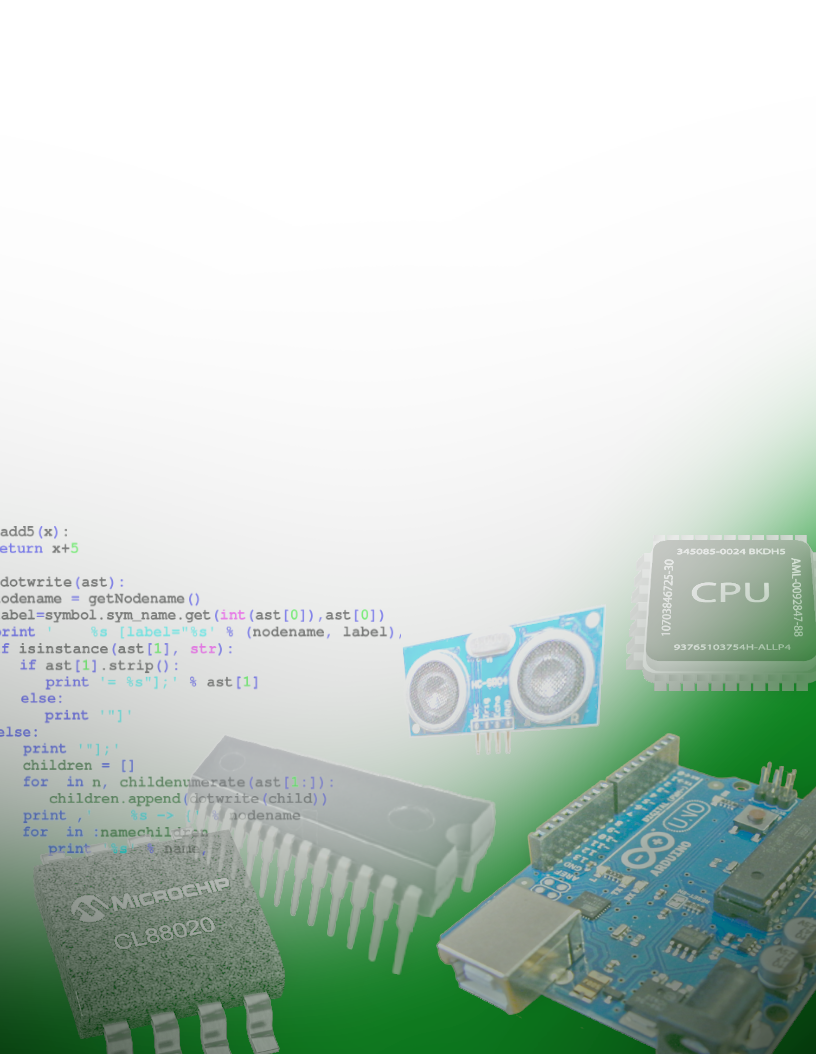
\includegraphics[scale=1.01]{FONDO.png}
 }
}

\begin{document}
\begin{titlepage}
\BgThispage
\newcommand{\HRule}{\rule{\linewidth}{0.5mm}}
\center

\includegraphics[scale=0.4]{Escudo.jpg}\\[0.5 cm]
\textsc{\large Departamento de electrónica}\\[0.5cm]
\textsc{\large Curso de informática II}\\[0.5cm] 
\HRule \\[0.4cm]
{ \huge \bfseries Proyecto de investigación: \\[0.5 cm]\LARGE Interrupciones en el campo de microprocesadores}\\[0.4cm]
\large{por: }\\[0.3cm]
\textsc{Santiago Giraldo Tabares}\\
\HRule \\[1.5cm]
{\LARGE{Medellín, Antioquia, Colombia\\[0.2 cm]Julio, 2020}}\\
\vfill
\end{titlepage}


\begin{multicols}{2}

\section*{¿Qué son las interrupciones en microprocesadores?}
Son, como su nombre indica, el cese de las tareas que se estén realizando en el procesador (rutina), con el fin de atender otra tarea tangente a su funcionamiento principal (subrutinas). Son solicitudes/señales que recibe el procesador para atender tareas específicas. Estas solicitudes pueden provenir de periféricos externos y de manera inesperada, o de un algoritmo y de forma pre-programada. Podemos hacer una analogía con una situación cotidiana: En un aula, un alumno levanta la mano interrumpiendo el transcurso de la clase, con el fin de que el maestro resuelva una duda puntual. En este caso, la rutina sería la clase, la interrupción sería el levantamiento de la mano y la subrutina constaría de resolver la duda. Una vez resuelta la inquietud, el maestro continúa con la clase. (Para profundizar a nivel técnico, ver \cite{Ruz})
\section*{¿Se puede hablar de la historia de las interrupciones?}
Se puede hablar de la historia de las interrupciones en tanto que se hable de la historia de los microprocesadores. La idea de las interrupciones podemos verla aplicada hasta en el primer microprocesador, el 4004 de Intel (desarrollado en 1971) (estudiar el 4004 en \cite{Shi}. Recorrido historico en \cite{Mor}). Este realizaba un sondeo de todos los dispositivos esperando que alguno tuviese la configuración de bits que indicara que tenía una tarea para ser atendida. A esta técnica se la llama polling, y consta básicamente en preguntarle a todos los puertos/dispositivos, constantemente, si necesitaban atención para una tarea, y en caso de haber solicitudes de interrupción, atenderlas una a una (Profundizar en \cite{Chi}). Llevado a la analogía anterior, sería cómo si el profesor estuviera cada 2 minutos, preguntando a todos sus estudiantes, si tienen alguna duda puntual. Esto era algo ineficiente y con el tiempo, el polling sería desplazado progresivamente por las interrupciones que conocemos hoy. Denominadas con este mismo nombre, o en inglés, "interruption request", cambian el modelo de sondeo, por el de “aviso”, donde el procesador solo debe estar habilitado para recibir señales de interrupción, o como analizábamos antes, a que el estudiante levante la mano. Esto aumenta el costo a nivel Hardware pero es más rápido. Este cambio de mecanismo fue progresivo y es difícil datar un punto histórico exacto, sin embargo podríamos mencionar procesadores como el Intel 8080 e Intel 8085 \cite{Qui}, que fueron de los primeros en implementar el chip controlador de interrupciones (PIC) Intel 8259 \cite{Int2}, quien proveía al procesador con 15 canales de interrupción mediante los cuales el resto del hardware podía enviar sus solicitudes (datasheet 8080 \cite{Int} y sobre los PIC en \cite{Wai}).
\section*{Tipos de interrupciones: }
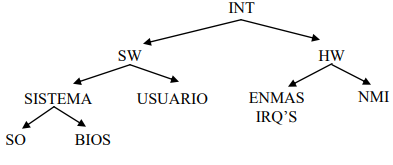
\includegraphics[scale=0.7]{tipos de interrupciones.PNG}\\[0.5 cm]
*Clasificaciones. Referencia a la imágen: \cite{Bel}*\\
Existen de forma general, y según su proveniencia, dos tipos de interrupciones. Las interrupciones por hardware y las interrupciones por software.
\section*{Por Software: }
Son solicitudes enviadas por un programa en ejecución, por lo tanto, su origen radica en el mismo procesador. Dado lo anterior, se les denomina “internas”, pues un algoritmo en ejecución llega a una orden propia que lo obliga a pausar su curso y a llamar al S.O para que se gestione la realización de otra tarea externa. Se dice que son programables dado a que están explícitas en el código fuente del algoritmo en ejecución.\\\\
\indent En estas, cabe aclarar que tanto el lenguaje del programa como el hardware utilizado IMPORTAN y afectan la implementación, dado que cada lenguaje utiliza sus propias palabras reservadas y funciones para enviar la petición de interrupción a un determinado canal y dadas ciertas condiciones o ciertos parámetros para la funciones. Además, el hardware debe estar adecuado con los suficientes canales de gestión de interrupciones, y debe consonar con las expectativas del lenguaje a utilizar. También afecta la cercanía del lenguaje utilizado con el lenguaje de máquina. En varios tipos de interrupciones es primordial la velocidad de atención, por lo tanto los lenguajes de bajo nivel ofrecen una ligera ventaja en ese aspecto. También, cuanto más se avanza en la miniaturización de los microprocesadores, también se avanza tanto en la velocidad de emisión de las peticiónes como en la de la ejecución de las subrutinas. También hay microprocesadores que tienen excepciones propias dadas la arquitectura de su ISA como su arquitectura física, así que en conclusión, el hardware y software utilizados marcan la diferencia.
\section*{Por Hardware: }
 Son provenientes de periféricos externos, como por ejemplo, dispositivos de entrada y salida. Dado lo anterior, se les denomina “externas”, y debido a su naturaleza, no son eventos programados, ergo, pueden ocurrir en cualquier momento. Consideremos el trabajo de  construcción de un edificio: Pueden ocurrir fallos inesperados, pero por ejemplo: las escaleras del piso 5 no están programadas para derrumbarse a las 2 semanas de comenzada la construcción, no es propio de su naturaleza y dependerá de factores externos.
 \subsection*{Excepciones: }
Existe otro tipo de interrupciones que podríamos calificar como internas. Hablamos de las excepciones. Las excepciones son interrupciones que se originan de las instrucciones anormales del lenguaje del algoritmo. En otras palabras, son aquellas que detienen y abortan el programa en ejecución por una instrucción mal construída, como las divisiones entre cero, violación de privilegios, error de los canales, instrucciones ilegales, etc. Son sincrónicas, pues se presentan en el momento exacto en el que el procesador llega a determinada instrucción y procede a dar un tratamiento que generalmente termina en la notificación al usuario/sistema y con el aborto de la ejecución, reanudando la rutina previa (ver \cite{Upm}).
 \subsection*{Por Timer: }
Así mismo, podríamos mencionar un subtipo de las interrupciones por software, bastante específico y de uso común en microcontroladores. Hablamos de los timers. Estos permiten que las instrucciones de un algoritmo se ejecuten en un tiempo planificado y no a la vertiginosa velocidad de nuestro procesador. Permite generar pausas y su utilización puede varíar (o de plano, existir) dependiendo del lenguaje de programación utilizado y la compatibilidad de nuestro hardware. Estas nos permiten, por ejemplo, controlar el tiempo de ejecución de un algoritmo mientras se ejecuta otra tarea en paralelo de forma constante. A nivel practico, podríamos encender y apagar un LED cada n segundos y tener otro algoritmo ejecutandose normalmente en segundo plano (un Buzzer, por ejemplo). Hay funciones como las de la librería TimerOne.h en arduino, las cuales permiten manipular estos timers para interrumpir, por periodos de tiempo controlados, una labor.

\section*{Clasificación según la prioridad de su solicitud:}
Las anteriores no son las únicas formas de categorizar las interrupciones. Tambien podemos clasificar las solicitudes de interrupción (no tanto LAS interrupciones como tal) según si son o no ignorables, proviniendo de un periferico Hardware.

\subsection*{Enmascarables:} 
Cuando el procesador recibe una petición de interrupción, este está en capacidad de apoyarse del software para decidir si ignorar o no esta petición, continuando con el curso normal de ejecución. En el registro de estatus (FLAG REGISTER) del procesador, o más específicamente, del controlador de interrupciones que este tiene, deben estar habilitadas las interrupciones cambiando el estado binario de un bit que hace de bandera o switch para cada canal de interrupciones. El estado de dicho bit puede ser manipulado por el usuario con instrucciónes de software. Se pueden inhibir todos los canales de interrupción o también se pueden inhibir canales de manera individual. Estas permiten que el controlador de interrupciones las pueda filtrar y administrar según la prioridad que requieran sus periféricos emisores, haciendo eficiente la gestión de los limitados canales de interrupción y permitiendo que la capacidad multi-tarea de los microprocesadores no se desborde provocando daños, paradas o ineficiencia.

\subsection*{No enmascarables:} 
Este tipo de solicitudes de interrupción son aquellas que no pueden ser interrumpidas y el procesador si o si debe efectuar la subrutina correspondiente para tratarla. Estas son especialmente útiles cuando el tiempo de respuesta a una tarea externa debe ser inmediato, de primerísima prioridad y en situaciones críticas que requieran tratamiento no solo obligatorio, sino rápido.\\[1 cm]
*Referencia sobre las anteriores clasificaciones en \cite{Bel}
\section*{Clasificación según método de asignación de subrutina: }
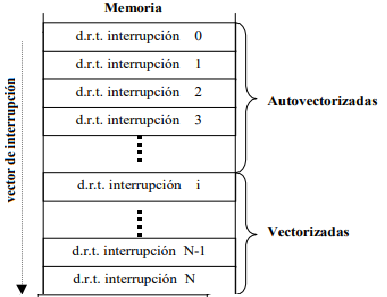
\includegraphics[scale=0.7]{tabla de vectores.PNG}\\
*Referencia a la imágen: \cite{Ruz2}*\\[0.5 cm]
Por último, también podemos llegar a  toparnos con términos que aluden a la forma en la que se conectán las peticiónes recibidas con las subrutinas o tratamientos que deben llevarse a cabo. En la memoria del computador, se encuentra almacenado un vector de interrupciones que almacena en cada una de sus posiciones, las direcciones de memoria de cada una de las subrutinas que debe ejecutar el procesador ante cada solicitud específica. a continuación se explica en que forma pueden llegar las peticiones de interrupción:
\subsection*{No vectorizadas: }
Estas, también llamadas 'Autovectorizadas', son aquellas a las que el periferico emisor de la petición no les ha asignado un vector de interrupción, por lo tanto debe ser el procesador quién, a través de software, asigne un canal para que dicha solicitud pueda ser procesada. El procesador también debe inspecciónar el periferico emisor para determinar la prioridad de la petición.

\subsection*{Vectorizadas: }
Son aquellas que sí cuentan con un vector de interrupción. Una vez se reconoce la interrupción al dispositivo externo, este asigna el vector a la solicitud, con lo que llegará a una determinada posición en memoria para que el procesador pueda proceder luego con la subrutina correspondiente.
\\\\Referencia a vectorización en \cite{Ruz2}

\section*{Ejmplo de implementación:}
A continuación, se adjunta el link a una simulación en Tinkercad elaborada para ejemplificar una interrupción externa sobre una placa Arduino UNO R3, con la respectiva explicación del código fuente: \url{https://www.tinkercad.com/things/g2QTusrjTsS}.\\\\
\end{multicols}
\begin{thebibliography}{x}
\bibitem{Ruz} \textsc{Ruz Ortíz, J.J.}
\textit{Tema 9: interrupciones}, Dpto. de Arquitectura de Computadores y Automática, Facultad de Informática,  Universidad Complutense de Madrid.\\\url{http://www.fdi.ucm.es/profesor/jjruz/WEB2/Temas/Curso05_06/EC9.pdf}

\bibitem{Qui} \textsc{Quintero Reyes, A.G.}
\textit{interrupciones}, [Archivo de video], recuperado de \\\url{https://www.youtube.com/watch?v=bIXYtXL587M}. Fuente verificada en \url{https://repository.unad.edu.co/handle/10596/5356}

\bibitem{Shi} \textsc{Shima, M.}
\textit{The 4004 CPU of My Youth: Developing the world’s first microprocessor.}, IEEE SOLID-STATE CIRCUITS MAGAZINE, (Winter, 2009). \\\url{https://ieeexplore.ieee.org/stamp/stamp.jsp?arnumber=4776533}

\bibitem{Chi} \textsc{Chishti, Z.}
\textit{Microprocessor System Design}Electrical and Computer Engineering Dept, Maseeh College of Engineering and Computer Science, Portland State University \\\url{http://web.cecs.pdx.edu/~zeshan/ece585_lec3.pdf}

\bibitem{Int} \textsc{Intel}
\textit{8080A/8080A-1/8080A-2. 8 bit N-channel microprocessor [official datasheet]}\\\url{http://www.datasheetcatalog.com/datasheets_pdf/8/0/8/0/8080.shtml}

\bibitem{Mor} \textsc{Morse, S.P. Ravenel, B.W. Mazor, S. Pohlman, W.B.}
\textit{Intel Microprocessors: 8008 to 8086}, IEEE Computer, Vol 13, No. 10, pages 42-60, October 1980 pp. 73-74. \\\url{http://stevemorse.org/8086history/8086history.doc}

\bibitem{Int2} \textsc{Intel}
\textit{8259A PROGRAMMABLE INTERRUPT CONTROLLER (8259A/8259A-2) [Official datasheet]} \\\url{https://pdos.csail.mit.edu/6.828/2005/readings/hardware/8259A.pdf}

\bibitem{Ruz2} \textsc{Ruz Ortiz, J.J.}
\textit{Tema 3. Entrada/salida programada e interrupciones}, Dpto. de Arquitectura de Computadores y Automática, Facultad de Informática,  Universidad Complutense de Madrid.\\\url{http://www.fdi.ucm.es/profesor/jjruz/EC-IS/Temas/Tema%203-%20Entrada_salida%20programada%20e%20interrupciones.pdf}

\bibitem{Wai} \textsc{Wainer, G.A.}
\textit{The Programmable Interrupt Controller}, SYSC-3006* - Computer Organization, Department of Systems and Computer Engineering, Carleton University (Fall, 2011). \\\url{http://www.sce.carleton.ca/courses/sysc-3006/f11/Part18-PIC.pdf}

\bibitem{Bel} \textsc{Beltrán Martínez, B.}
\textit{Ensamblador. Interrupciones},Ciencias de la Computación, Benemérita Universidad Autónoma de Puebla, México. \\\url{http://bbeltran.cs.buap.mx/Interrupciones.pdf}

\bibitem{Upm}
\textit{PRÁCTICAS DE MICROPROCESADORES PRÁCTICA V. “MANEJO DE EXCEPCIONES”. Implementación de un reloj},DPTO. ELECTRÓNICA, AUTOMÁTICA E INFORMÁTICA INDUSTRIAL, Universidad Politécnica de Madrid, España. \\\url{http://www.ieef.upm.es/webantigua/spain/Asignaturas/Microprocesadores2002/practicas/up-p5.pdf}

\bibitem{San} \textsc{Santamaría, E.}
\textit{Microprocesador 68000: Hardware y Software}, Universidad Pontificia de Comillas(pp. 22 - 25). \\\url{https://books.google.com.co/books?id=Us64bLlWh54C&printsec=frontcover#v=onepage&q&f=false}

\bibitem{Val} \textsc{Valdés Peres, F.E. Pallás Areny, R.}
\textit{Microcontroladores Fundamentos y Aplicaciones con PIC}, Universidad de Oriente, Cuba. Universidad Politécnica de Cataluña, España, 2007.(pp. 217 - 218). \\\url{https://books.google.com.co/books?id=ODenKGOHMRkC&printsec=frontcover#v=onepage&q&f=false}

\bibitem{Bur} \textsc{Burgess, P.}
\textit{Adafruit NeoPixel Überguide} [Guía oficial de uso de las librerías de Adafruit Neopixel][referencia del uso de la implementación en Arduino]\\\url{https://learn.adafruit.com/adafruit-neopixel-uberguide/arduino-library-use}

\end{thebibliography}

\end{document}